\documentclass[10pt]{article}
\usepackage[margin=0.7in]{geometry}
\usepackage[T1]{fontenc}
\usepackage{graphicx}
\begin{document}
\section*{Independent ordinary Kummer fiber review}
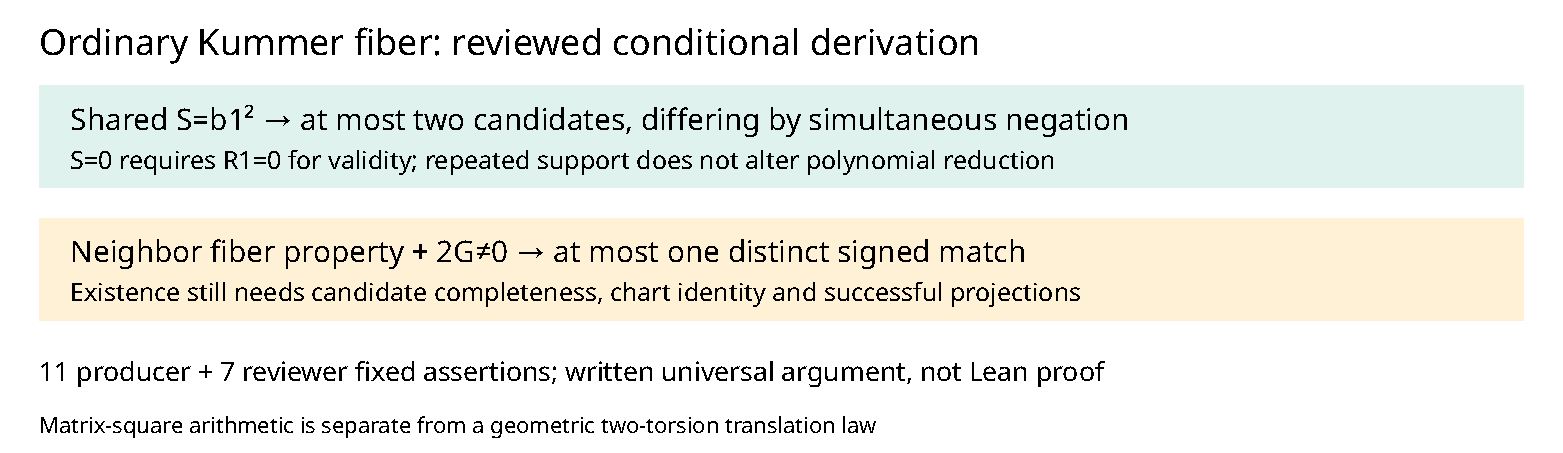
\includegraphics[width=\linewidth]{flow.pdf}
\paragraph{Result.} Validated at the stated scope as a written derivation. This is not a universal Lean theorem or verification of all native coordinate formulas.
\paragraph{Fiber and zero square.} Reducing $(b_0+b_1X)^2$ modulo $X^2+a_1X+a_0$ yields the stated two equations without requiring squarefree support. Assuming the shared square identity and a valid divisor, nonzero $S$ fixes $b_1$ up to sign and then $b_0$ uniquely in characteristic other than2. For $S=0$, $b_1=0$ and validity requires $R_1=0$; the source generates candidates before applying this validity filter. Global deduplication limits the generated vector to two distinct candidates even though the zero branch is visited twice.
\paragraph{Neighbor and geometry.} The neighbor argument proves uniqueness under the quotient-fiber property on the neighbor domain and $2G\ne0$. The alternative $2D=0$ identifies the two candidates. Existence separately needs coordinate correctness, candidate completeness and successful projections. Ordinary-chart algebra does not cover boundary neighbor charts automatically. Matrix-square arithmetic proves invertibility, not translation by a specified two-torsion point.
\paragraph{Native controls.} Eleven producer assertions and seven independent assertions passed fresh Rust runs. Reviewer checks include inconsistent $S=0$ residual, repeated support and characteristic2 denominator. These fixed checks are illustrative, not universal geometric evidence. One initial build had ambiguous integer literal types; failed source/stderr and absent-binary invocation remain. Explicit i64 literals and fail-closed replay corrected the setup.
\paragraph{Custody and scope.} Source is pinned to publication125c631e4005785e344167d8f699b4bf23415fe6. Prior graph/polynomial familiarity is disclosed, without a blind-review claim. See REVIEW.md, status.json, receipt.json and replay.sh. No enumeration, curve computation, timing, scientific execution, repository edit, cloud operation or Python research occurred.
\end{document}
